\graphicspath{{./background/}}

\chapter{Background}
% {{{
\label{cha:background}

% {{{

Information visualisation techniques are very domain specific; one type of
visualisation may work well for a particular scenario, but work quite poorly
when applied to another domain. The problem domain of this project is the
effective visualisation of point cloud data, more specifically, water molecules
from molecular simulations.

As water is the solvent in molecular simulations, it occupies much of the
volume. This poses the challenge on how to effectively visualise large amounts
of point data. Some of the important issues that need to be investigated are
the presentation of appropriate levels of detail and clutter control.

Section \ref{sec:background_molecular} identifies and briefly introduces
several molecular visualisation techniques, while Section
\ref{sec:background_general} focuses on more general visualisation techniques.
Section \ref{sec:background_summary} provides a short summary of the different
visualisation techniques.

% }}}

\section{Molecular visualisation}
% {{{
\label{sec:background_molecular}

% {{{

The most significant problem for visualising molecular data is the amount of
data available and how to represent it so as not to clutter up the display.
Some molecular visualisation techniques focus on simplifying the models by
analysing the data to identify structures, while others exclude certain data
from the visualisation. Either way, a simplified image is presented so as to
make the molecular data easier and quicker to understand.

Some of the visualisation techniques (ribbon, paper chain and twister) are
designed for very specific molecular data, and are thus not easily extensible
to point cloud data. They can, however, be used as an example to determine what
kind of analysis can be done on data to simplify and help identify structures.

It is worth mentioning the Visual Molecular Dynamics (VMD) \citep{humphrey96}
program, it is a commonly used visualisation package aimed at displaying,
animating and analysing large biomolecular systems \citep{VMD}. However, as VMD
is aimed at general biomolecular systems, support for specific visualisation
and filtering is limited. VMD does support and use some of the visualisation
techniques that are mentioned in this chapter.

% }}}

\paragraph{Ball-and-stick}
% {{{

The ball-and-stick model is the classical approach to representing molecular
structure. Colour coded spheres are used to represent the atoms, while
cylinders are used to represent the bonds between them. There are various
proposals for the colour scheme used in ball-and-stick representations
(\citep{rasmolcolour}, \citep{jmolcolour}, \citep{drumscolour}), but there is
no definite agreed upon standard. This model is used to emphasise the molecular
connectivity of the atoms. It is the one of the simpler approaches in molecular
visualisation and is most often used when much detail is required: typically
for looking at bond information, molecule orientation and reaction sites.

The problem with this model is that it does not handle large numbers of atoms
and bonds very well. Since all the atoms and bonds are visible, the view
quickly becomes crowded and overall structure is obscured. Occlusion of other
atoms often occurs and may hide important information. The ball-and-stick
representation is typically not used for large structures as it often produces
cluttered views, making it very difficult to understand and analyse the data.

% }}}

\paragraph{CPK}
% {{{

The CPK (Corey-Pauling-Koltun) \citep{corey53} representation simplifies the
ball-and-stick model by removing the cylinders used to represent bonds. The
spheres used for the atoms are enlarged to encompass the bonds. The atoms now
overlap with one another, covering up where the bonds would be.

Removing the bonds from the model simplifies the view and allows for the
overall shape and contour to be easily seen. Although this model has simplified
the ball-and-stick model, it does not highlight any structures, it has only
removed the bond information. In contrast, the later molecular visualisation
techniques in this section do highlight certain molecular structures.

The CPK representation is not well suited to the visualisation of large numbers
of molecules. As each of the atoms has been enlarged, each molecule occupies
more space than the ball-and-stick model; with the molecules being opaque, this
causes large areas to be occluded, which may hide important information and
make it hard to analyse an entire system.

Figure \ref{fig:background_ball_cpk} shows the ball-and-stick and CPK
representation of the same molecule. The ball-and-stick representation is on
the left, while the CPK representation is on the right.

\begin{figure}
  \begin{center}
    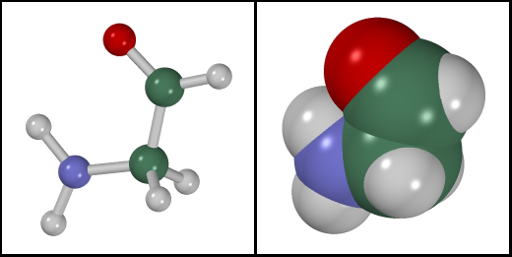
\includegraphics[width=100mm]{ball_cpk}
  \end{center}
  \caption{Ball-and-stick (left) and CPK (right) representations of the same
  molecule.}
  \label{fig:background_ball_cpk}
\end{figure}

% }}}

\paragraph{Solvent accessible surfaces}
% {{{

Solvent accessible surfaces \citep{connolly83} produces a similar effect to
CPK. The bonds are not visible and the atoms are enlarged, the difference lies
in the approach taken to produce the surface of the volume. The solvent
accessible surface is created by determining where the solvent (modelled using
spheres) can and cannot fit.

Figure \ref{fig:background_sas} is a schematic diagram illustrating how the
solvent accessible surface is determined. The molecular surface is marked in
purple. Even though the surface of the molecule (CPK representation) has many
crevasses, the solvent (the circles labelled with an `S') cannot fit in them and
thus the boundary is extended to where the solvent can fit.

\begin{figure}
  \begin{center}
    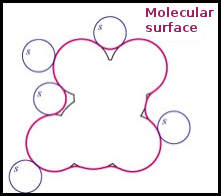
\includegraphics[width=60mm]{sas_ms}
  \end{center}
  \caption{Schematic diagram illustrating solvent accessible surfaces.}
  \label{fig:background_sas}
\end{figure}
% }}}

\paragraph{Protein molecules}
% {{{

The ribbon model (\citep{richardson81}, \citep{carson87}) was designed to
highlight the structure of protein molecules by fitting a curved surface to the
backbone of the molecule. This allows for the shape of the protein molecule to
be easily seen and followed.

Figure \ref{fig:background_ribbon} shows the backbone of a protein, the oxygen
atoms of the protein backbone are used to determine the normal for drawing the
oriented ribbon.

This has proved to be highly effective at highlighting the structure of
proteins. Unfortunately, this approach is not as effective when applied to
non-protein molecules such as carbohydrates and lipids, where the molecular
structure is different. Thus, the traditional ball-and-stick and CPK models are
still widely used for carbohydrate and lipid visualisation.

\begin{figure}
  \begin{center}
    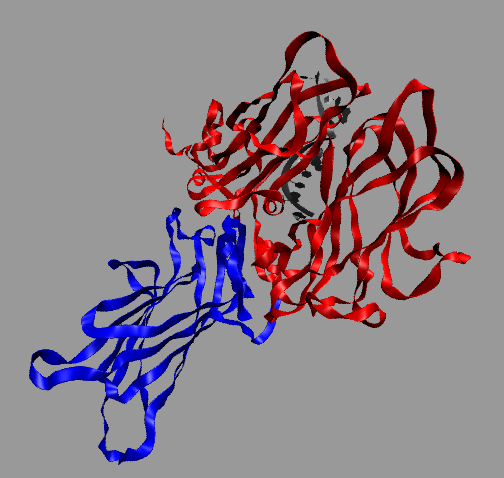
\includegraphics[width=60mm]{ribbon}
  \end{center}
  \caption{Ribbon model of a protein.}
  \label{fig:background_ribbon}
\end{figure}

% }}}

\paragraph{Carbohydrate molecules}
% {{{

The paper chain visualisation technique \citep{kuttel06} focuses on
highlighting ring structures in carbohydrate molecules. Ring structures are
first identified and are then displayed using a ring polyhedron.

This significantly simplifies the carbohydrate molecules by only showing the
carbohydrate rings, which would otherwise have been obscured in other
visualisations (ball-and-stick and CPK). The ball-and-stick model can still be
overlayed on the paper chain view to provide detailed information if needed.

The twister visualisation technique \citep{kuttel06} builds on the paper chain
technique by highlighting the relative orientations of the identified
carbohydrate rings. Each carbohydrate ring is represented by a disc, which is
then connected to another disc with a ribbon. The ribbon follows the
orientation from one ring to another, thus showing how the rings are connected
to one another.

The twister visualisation technique is similar to the ribbon model for proteins
in that it shows the overall shape of the molecule quite effectively. And, as
with the ribbon model, this visualisation technique is designed for a specific
type of molecule.

Figure \ref{fig:background_chain_twister} shows the paper chain and twister
models. The respective ball-and-stick representations of the carbohydrates are
overlayed semi-transparently over the models.

\begin{figure}
  \begin{center}
    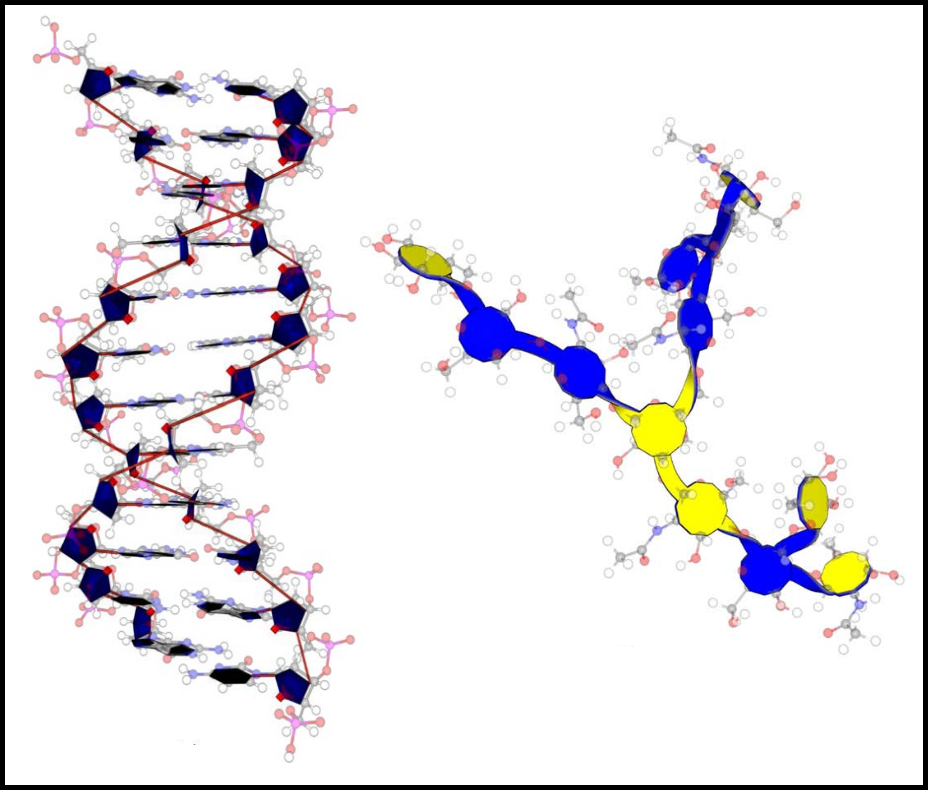
\includegraphics[width=100mm]{chain_twister}
  \end{center}
  \caption{Paper chain (left) and Twister model (right) of a carbohydrate, with
  ball-and-stick model overlayed semi-transparently.}
  \label{fig:background_chain_twister}
\end{figure}

% }}}

\paragraph{Summary}
% {{{

The different visualisation techniques discussed in this section are summarised
in Table \ref{tab:background_molecular}. The ball-and-stick representation is
used as the baseline for comparing against the other techniques. The table
lists the different molecular visualisation techniques, indicates the molecule
type that they are specific to, and whether they summarise the structure of the
molecule or not.

\begin{table}
  \begin{tabular}{ | l | l | l | }
  \hline
  Technique                   & Molecule type & Summarisation of structure?  \\ \hline
  Ball-and-stick              & All           &                              \\ \hline
  CPK                         & All           & A little                     \\ \hline
  Solvent accessible surfaces & All           & A little                     \\ \hline
  Ribbon                      & Protein       & Yes                          \\ \hline
  Paper chain                 & Carbohydrate  & Yes                          \\ \hline
  Twister                     & Carbohydrate  & Yes                          \\ \hline
  \end{tabular}
  \caption{Table summarising the molecular visualisation techniques, what
  molecule types they are specific to and do they summarise the structure.}
  \label{tab:background_molecular}
\end{table}

% }}}

% }}}

\section{General visualisation}
% {{{
\label{sec:background_general}

% {{{

The more relevant techniques from general visualisation with regards to point
cloud data are: surface extraction, volume rendering and general clutter
control techniques. Mesh decimation and metaballs are also relevant, but they
have more specific uses.

% }}}

\paragraph{Surface extraction}
% {{{

The marching cubes algorithm \citep{lorensen87} is the classical approach for
surface extraction. The algorithm works by sampling a 3D volume (voxelising the
volume) and then examining each voxel in the data to determine whether it is
inside the volume or not. A surface can then be determined by combining all the
voxels which intersect with the volume boundary. Figure
\ref{fig:background_mesh} shows the extracted surface of a skull.

Marching tetrahedrons is an alternative surface extraction algorithm to
marching cubes. Instead of using a cube as the sampling structure, a
tetrahedron is used. Each voxel in the data is split into 6 tetrahedrons, which
are used to determine whether that voxel intersects with the volume boundary.

Surface extraction allows for the shape of the volume to be extracted and
visualised, and is somewhat analogous to the CPK model in that regard. It can
be adapted to molecular data to provide a simpler, smoothed view of the
molecule, thus allowing for shape and contours to be more easily seen; which
may have otherwise been obscured by the details of the atoms.

The granularity of the sampling grid has a large impact on the quality of the
extracted surface. A grid where each individual voxel is quite small will
produce a detailed surface, but will correspondingly produce a large number of
polygons but these can be simplified away by mesh simplification. Section
\ref{sec:background_decimation} provides more detail on reducing the number of
polygons used to represent a surface.

\begin{figure}
  \begin{center}
    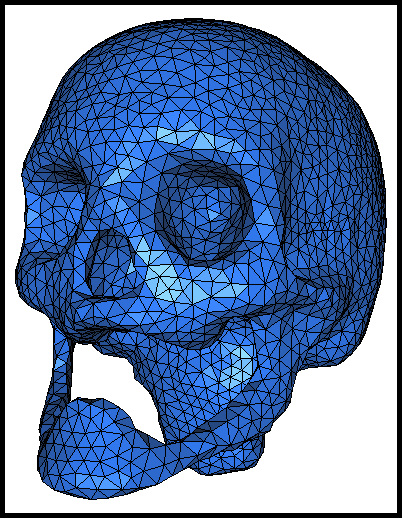
\includegraphics[width=50mm]{surface_mesh}
  \end{center}
  \caption{Extracted surface of a skull.}
  \label{fig:background_mesh}
\end{figure}

% }}}

\paragraph{Volume rendering}
% {{{

Volume rendering aims to visualise the entire volume instead of an object's
surface. The data is modelled as a translucent gel where one is able to see
through the volume, while still being able to see what is inside the volume.
Figure \ref{fig:background_head} is a ray cast image of a head. The internal
bones are clearly visible through the translucent skin and flesh.

There are two main approaches to volume rendering. The first works from the
image plane to the volume, and is called image order processing. Ray casting is
the typical approach to this problem as proposed by Levoy \citep{levoy88}. The
second approach, object order processing works from the volume to the image
plane. The classical approach to this is splatting \citep{westover89}. Hybrid
methods have been developed to take advantage of both approaches.

The main advantage of volume rendering is the ability to visualise the entire
volume at once, but this demands increased complexity and computation. Volume
rendering is not directly applicable to molecular data, but it can provide an
aggregated view of the entire volume.

\begin{figure}
  \begin{center}
    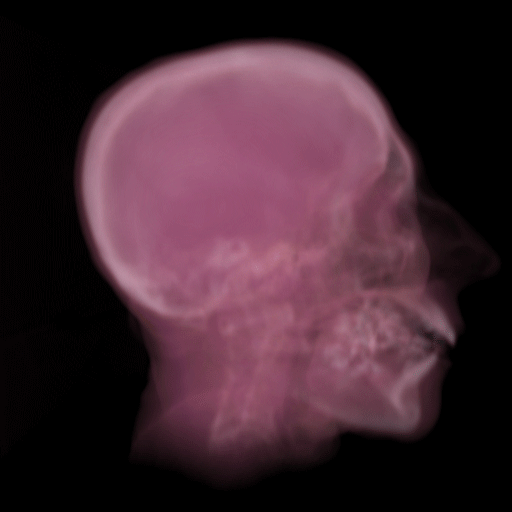
\includegraphics[width=70mm]{head_volume}
  \end{center}
  \caption{Ray cast image of a head.}
  \label{fig:background_head}
\end{figure}

% }}}

\paragraph{Clutter reduction}
% {{{
\label{sub:background_clutter}

Shneiderman provides a \emph{visual information-seeking mantra}
\citep{shneiderman96}: ``overview first, zoom and filter, then details on
demand'', which allows the consideration of clutter reduction techniques. The
methodology provides a general hierarchy of tasks to be applied to information
visualisation, in which clutter reduction plays an important role.

Ellis and Dix \citep{ellis07} provides a taxonomy cross referencing clutter
reduction techniques against certain criteria. With clutter reduction, a
trade-off between removing too much and too little information must be made.
Removing too much or too little data will produce a visualisation that is of
little use.

With regards to visualising point cloud data, \emph{filtering} \citep{stone94},
\emph{opacity} \citep{kosara02} and \emph{topological distortion}
\citep{lamping96} are the most useful clutter reduction techniques.

\emph{Filtering:} Only certain objects fulfilling certain criteria are
displayed in order to reduce clutter. The criteria can consider certain
characteristics or objects in a certain area or locus of interest; irrelevant
objects are removed. Uninteresting occluding objects are also removed to show
objects in important areas or with important characteristics.

Another approach to filtering is to highlight the important features of the
data with colour, but leave the rest of the data visibly unchanged. This has
the advantage of maintaining context.

Figure \ref{fig:background_highlight} is an example application of highlighting
in a graph structure. The more oftenly traversed paths are more important,
which is reflected in the colouring. From looking at the image, it is clear
that the intersection on the right edge of the image is the most heavily
traversed area of the graph as it is the brightest.

\emph{Opacity:} The translucency of items can be changed to highlight or hide
elements. This is similar to filtering, in that irrelevant items are partially
or entirely hidden, highlighting only the important parts. The advantage of
opacity over filtering is that other information is not entirely removed, it is
still available if needed and can be used to hint at contextual information.
Opacity can also be adapted to show temporal information, where the previous
frame is rendered along with the current frame, but at a lower opacity;
creating an effect similar to motion blur.

\emph{Topological distortion:} The representation of the data can be changed so
that certain areas are larger. This highlights and focuses on the relevant
areas, while de-emphasising the other areas. The distortion can either be
uniform (zooming), or can be non-uniform (fish-eye effect).

Clutter reduction techniques have the most potential for point cloud
visualisation as there is a need to be able to visualise many objects in 3D
space. However, care must be taken to not remove important and relevant
information. It should be noted that clutter reduction techniques are not all
mutually exclusive, many of the techniques complement one another.

\begin{figure}
  \begin{center}
    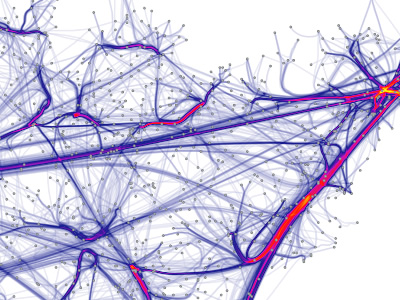
\includegraphics[width=70mm]{graph_highlight}
  \end{center}
  \caption{Colour is used to highlight highly traversed path.}
  \label{fig:background_highlight}
\end{figure}

% }}}

\paragraph{Metaballs}
% {{{

Metaballs \citep{blinn82} is a technique for producing organic-looking objects.
The metaballs volume is modelled using a number of points that exert forces
around themselves, the surface of the volume is determined by the set of points
where the force function is equal to some constant threshold value. The surface
is usually determined using surface extraction techniques.

There are 15 metaball points in Figure \ref{fig:background_metaballs}, the
metaball points are the roundish parts of the volume. Areas of the volume
appears to melt and blend together, yielding the blobbly appearance. The force
functions used takes into account the nearby metaball points, which causes the
merging effect.

The advantage of metaballs is that volume data is grouped together, making it
easy to see the different volumes in a region. The disadvantage of this
technique is the computational cost required to determine and extract the
surface from the force calculations.

\begin{figure}
  \begin{center}
    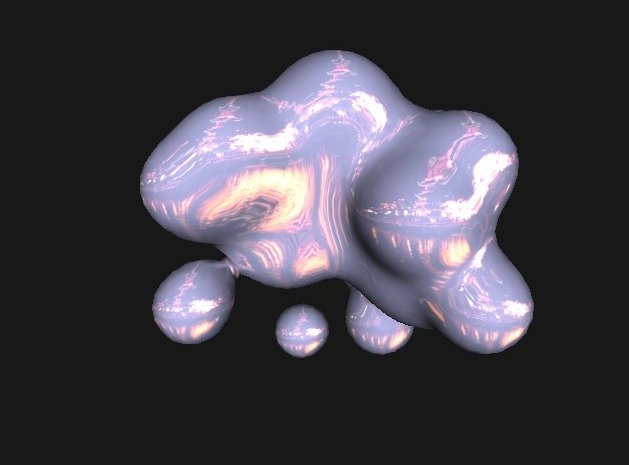
\includegraphics[width=70mm]{metaballs}
  \end{center}

  \caption{A volume determined with 15 metaballs exerting forces around
  themselves.}

  \label{fig:background_metaballs}
\end{figure}

% }}}

% }}}

\section{Mesh decimation}
% {{{
\label{sec:background_decimation}

The amount of time taken to render a model is proportional to the number of
polygons in the model. There is thus a trade-off between detail and render
time: more polygons will increase the amount of detail present, but will also
increase render time. Mesh decimation is a technique aimed at reducing the
number of polygons used to represent a mesh while preserving as much detail as
possible.

Mesh decimation can be broadly divided into two main categories:
\emph{geometric decimation} and \emph{vertex clustering}. A more complete
comparison between mesh simplification algorithms can be found in Cignoni et
al. \citep{cignoni98}.

\paragraph{Geometric decimation}
% {{{

Geometric decimation iteratively eliminates components of the mesh: vertices,
edges or faces \citep{schroeder92}. The component to be removed is chosen using
local geometric optimality criteria. After eliminating the component, a local
re-triangulation process is used to fill in any resulting holes.

% }}}

\paragraph{Vertex clustering}
% {{{

Vertex clustering groups a number of geometrically similar and spatially close
vertices together \citep{rossignac93}, the group of vertices is then replaced
by a new representative vertex. Due to the simplicity of the test, vertex
clustering can be implemented very efficiently.

% }}}

% }}}

\section{Summary}
% {{{
\label{sec:background_summary}

This chapter has presented some visualisation techniques, each with their own
advantages and disadvantages. Visualisation techniques are best designed to
take advantage of specific domain knowledge. As a result, they are not easily
generalisable into other areas.

Molecular modelling is a specific instance of the scientific visualisation
problem, where the requirement is to be able to easily identify certain
structures. Different types of molecules each have their own specific
characteristics and structures. This knowledge can be exploited in the
different visualisation techniques: the ribbon representation is useful for
proteins, paper chain and twister for carbohydrates, while ball-and-stick and
CPK for general molecular visualisations.

General visualisation techniques address a slightly different problem: how to
visualise the data effectively and not necessarily to identify and highlight
specific structures. Thus the main concern is how to enable easy exploration of
the data.

None of the techniques touched on, handle time explicitly. If a temporal
dimension were to be added, all the techniques would simply treat each frame
separately and regenerate the visualisation given the new set of data. This
approach is not ideal if some interframe visualisation coherence is desired.

Visualising point cloud data, where there are many points in a region, is also
not very well handled. With water visualisation, the points are distributed
within a three dimensional volume, which makes visualisation more difficult.

There is no single solution for all visualisation needs. However, approaches
and ideas can be taken from different visualisation approaches. While the
problems may not be identical, there will be some overlapping requirements and
concerns.

% }}}

% }}}

